\documentclass{ctexart}
\usepackage{tikz}
\usepackage{xfp}
\usepackage{pgfplots}
\usetikzlibrary{arrows.meta}
\usetikzlibrary{shadings}
\newcounter{cnt}
\setcounter{cnt}{1}
\begin{document}
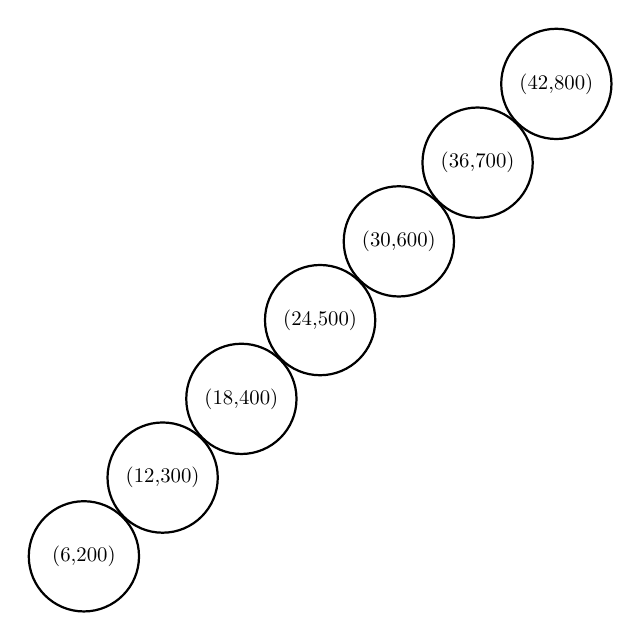
\begin{tikzpicture}
    \foreach \y[count = \x] in {2,3,...,8}{
            \draw[thick] (\x, \y) circle (.7cm) node [scale=.75] {($\fpeval{6*\x}$,$\fpeval{100*\y}$)};
        }
\end{tikzpicture}

比较\char 92 pgfmathsetmacro 与 \char 92 pgfmathtruncatemacro的显示区别

\begin{tikzpicture}
    \pgfmathsetmacro{\x}{2.0}
    \pgfmathsetmacro{\y}{3*\x+2}
    \pgfmathsetmacro{\xx}{\x+1}
    \pgfmathsetmacro{\yy}{\y+1}
    \draw(\x,\y) node[below] {(\x,\y)} -- (\xx,\yy) node[above] {(\xx,\yy)};
    \pgfmathtruncatemacro{\x}{1}
    \pgfmathtruncatemacro{\y}{2*\x+3}
    \pgfmathtruncatemacro{\xx}{\x+1}
    \pgfmathtruncatemacro{\yy}{\y+1}
    \draw(\x,\y) node[below] {(\x,\y)} -- (\xx,\yy) node[above] {(\xx,\yy)};
\end{tikzpicture}

\hspace{5cm}

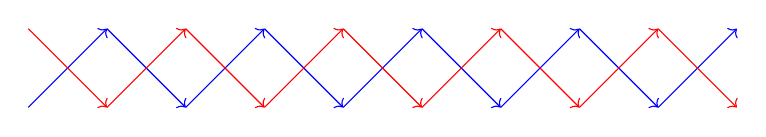
\begin{tikzpicture}
    \foreach \y[count=\x] in {0,1,0,1,0,1,0,1,0}{
            \draw[->,blue] (\x,\y) -- (\x+1,1-\y);
            \draw[->,red] (\x,1-\y) -- (\x+1,\y);
        }
\end{tikzpicture}

\hspace{5cm}

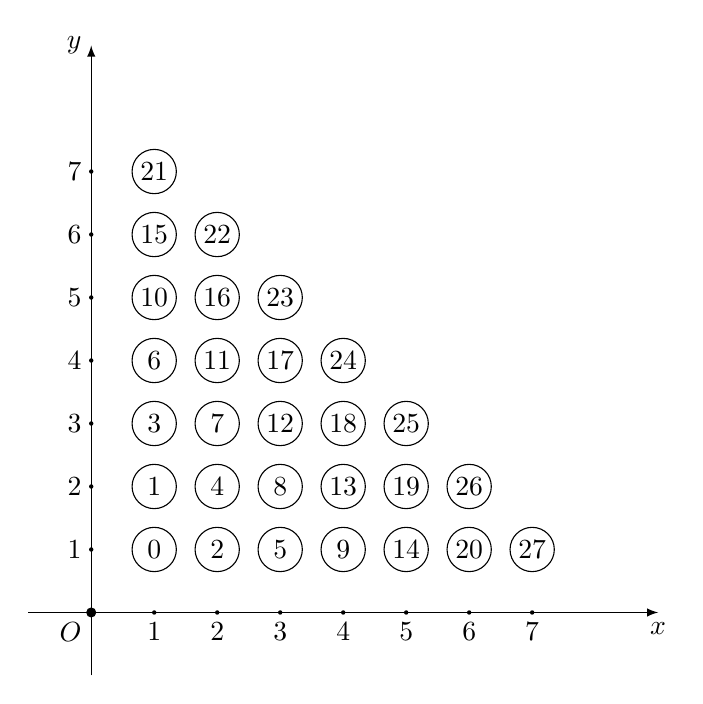
\begin{tikzpicture}[scale=0.8]
    % 使用了全局计数器 cnt 维护蛇形走位的计数
    \pgfmathsetmacro{\num}{0}
    \foreach \n in {1,...,7}{
            \foreach \x in {1,...,\n}{
                    \draw (\x,\n-\x+1) circle (10pt) node {\thecnt\global\stepcounter{cnt}};
                }
        }
    \draw[-latex] (-1,0) -- (9,0) node[below] {$x$};
    \draw[-latex] (0,-1) -- (0,9) node[left] {$y$};
    \foreach \i in {1,...,7}{
            \fill (\i,0) circle[radius=1pt] node[below] {\i};
            \fill (0,\i) circle[radius=1pt] node[left] {\i};
        }
    \filldraw (0,0) circle[radius=2pt] node[below left] {$O$};
\end{tikzpicture}

\hspace{5cm}

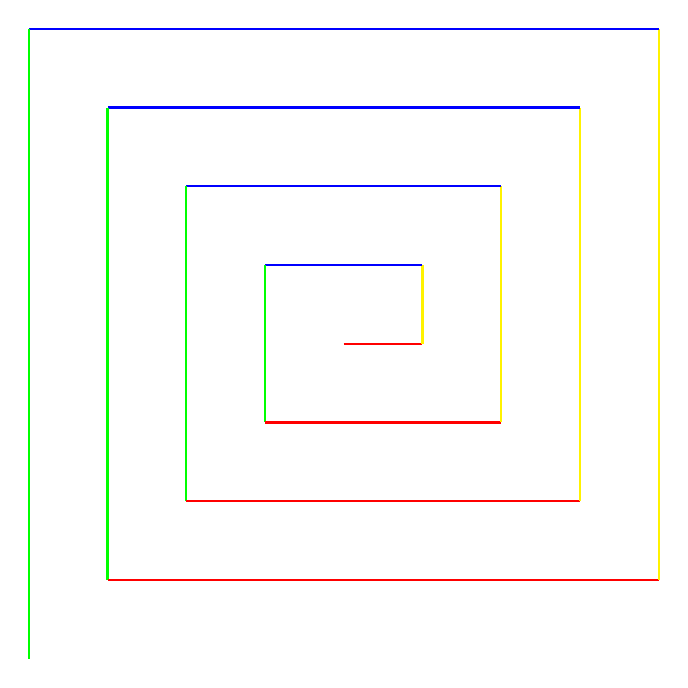
\begin{tikzpicture}
    \pgfmathtruncatemacro{\N}{4}
    \foreach \x[
        count=\n,
        evaluate=\n as \u using int(2*\n-1),
        evaluate=\n as \v using int(2*\n),
    ] in {1,...,\N}{
            %\draw (1-\n,1-\n) --++ (\u,0) --++ (0,\u) --++ (-\v,0) --++ (0,-\v);
            % \draw [thick,color = red] (1-\n,1-\n) --++ (\u,0);
            % \draw [thick,color = yellow] (1-\n+\u,1-\n) --++ (0,\u);
            % \draw [thick,color = blue] (1-\n+\u,1-\n+\u) --++ (-\v,0);
            % \draw [thick,color = green] (1-\n+\u-\v,1-\n+\u) --++ (0,-\v);
            \draw [thick,color = red] (1-\n,1-\n) --++(\u,0);
            \pgfgetlastxy{\macrox}{\macroy}
            \draw [thick,color = yellow] (\macrox,\macroy) --++ (0,\u);
            \pgfgetlastxy{\macrox}{\macroy}
            \draw [thick,color = blue] (\macrox,\macroy) --++ (-\v,0);
            \pgfgetlastxy{\macrox}{\macroy}
            \draw [thick,color = green] (\macrox,\macroy) --++ (0,-\v);
        }
\end{tikzpicture}


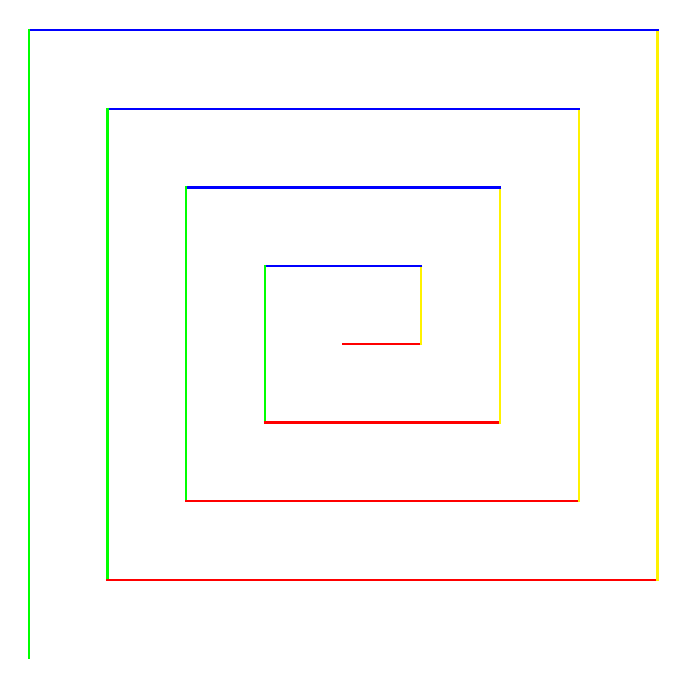
\begin{tikzpicture}
    \pgfmathtruncatemacro{\N}{4}
    \foreach \x[
        count=\n,
        evaluate=\n as \u using int(2*\n-1),
        evaluate=\n as \v using int(2*\n),
    ] in {1,...,\N}{
            % \draw (1-\n,1-\n) --++ (\u,0) --++ (0,\u) --++ (-\v,0) --++ (0,-\v);
            % \draw [thick,color = red] (1-\n,1-\n) --++ (\u,0);
            % \draw [thick,color = yellow] (1-\n+\u,1-\n) --++ (0,\u);
            % \draw [thick,color = blue] (1-\n+\u,1-\n+\u) --++ (-\v,0);
            % \draw [thick,color = green] (1-\n+\u-\v,1-\n+\u) --++ (0,-\v);
            \draw [thick,color = red] (1-\n,1-\n) --++(\u,0);
            \pgfgetlastxy{\macrox}{\macroy}
            \draw [thick,color = yellow] (\macrox,\macroy -.45pt) --++ (0,\u);
            \pgfgetlastxy{\macrox}{\macroy}
            \draw [thick,color = blue] (\macrox +.45pt,\macroy) --++ (-\v,0);
            \pgfgetlastxy{\macrox}{\macroy}
            \draw [thick,color = green] (\macrox,\macroy +.45pt) --++ (0,-\v);
        }
\end{tikzpicture}

\hspace{5cm}

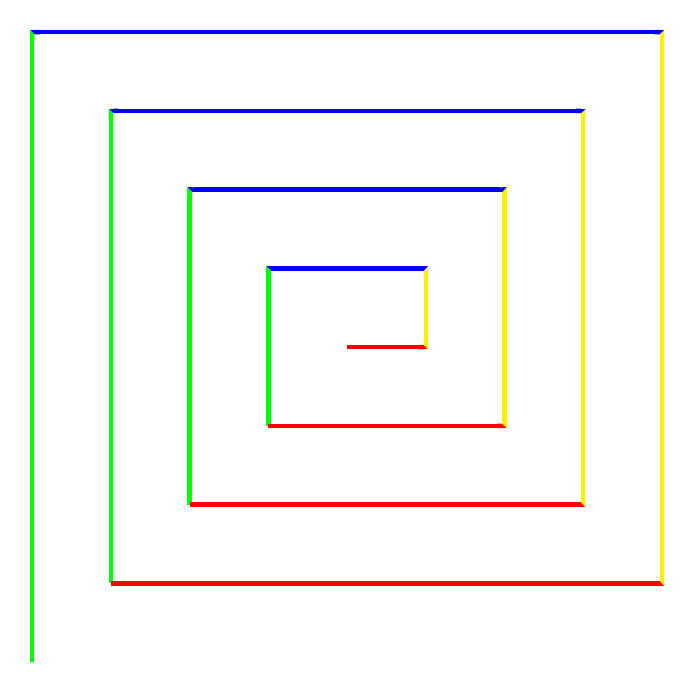
\begin{tikzpicture}[
    ultra thick,
    left/.tip={Butt Cap[sep=0pt -1]Rectangle[sep=0pt -0.5, slant=-1 ,width=0pt 1, length=0pt 2]},
    right/.tip={Butt Cap[sep=0pt -1]Rectangle[sep=0pt -0.5, slant=1 ,width=0pt 1, length=0pt 2]},
    ]
    \pgfmathtruncatemacro{\N}{4}
    \foreach \x[
        count=\n,
        evaluate=\n as \u using int(2*\n-1),
        evaluate=\n as \v using int(2*\n),
    ] in {1,...,\N}{
            \draw [color = red,-left] (1-\n,1-\n) --++(\u,0);
            \pgfgetlastxy{\macrox}{\macroy}
            \draw [color = yellow,right-left] (\macrox,\macroy) --++ (0,\u);
            \pgfgetlastxy{\macrox}{\macroy}
            \draw [color = blue,right-left] (\macrox,\macroy) --++ (-\v,0);
            \pgfgetlastxy{\macrox}{\macroy}
            \draw [color = green,right-] (\macrox,\macroy) --++ (0,-\v);
        }
\end{tikzpicture}

\hspace{5cm}

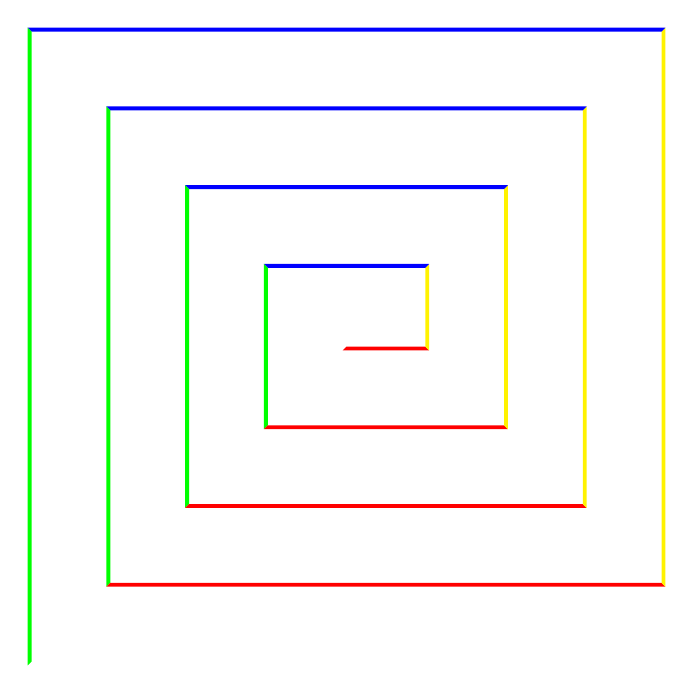
\begin{tikzpicture}
    \def\N{4}
    \def\Thickness{2pt}
    \foreach \x[
        count=\n,
        evaluate=\n as \u using int(2*\n-1),
        evaluate=\n as \v using int(2*\n),
    ] in {1,...,\N}{
            % 使用  coordinate (temp) 可以标记当前点 更方便绘图
            \fill [color = red] (1-\n,1-\n)--++(45:\Thickness)--++(\u,0) --++(-45:\Thickness) coordinate (temp) -- cycle;
            \fill [color = yellow] (temp)--++(135:\Thickness) --++ (0,\u)--++(45:\Thickness) coordinate (temp) -- cycle;
            \fill [color = blue] (temp)--++(-135:\Thickness)--++ (-\v,0)--++(135:\Thickness) coordinate (temp) -- cycle;
            \fill [color = green] (temp)--++(-45:\Thickness)  --++ (0,-\v)--++(-135:\Thickness) -- cycle;
        }
\end{tikzpicture}

\hspace{2cm}

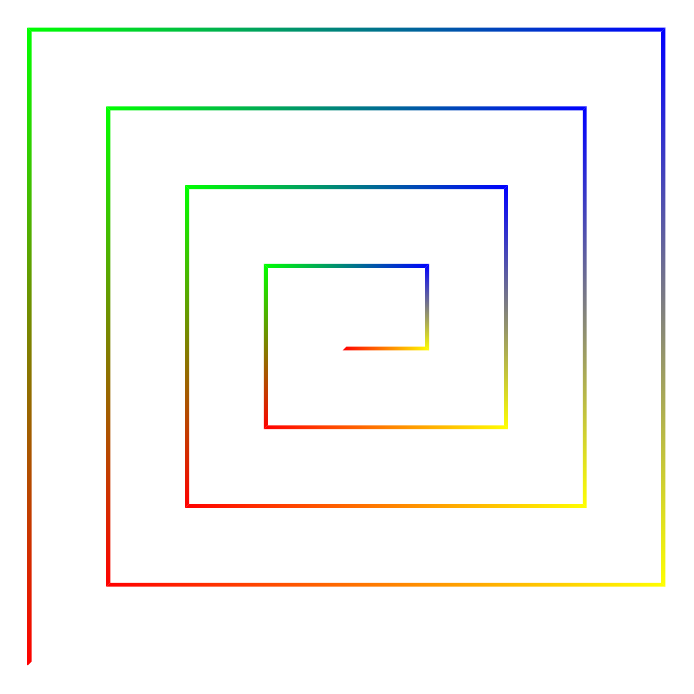
\begin{tikzpicture}
    \def\N{4}
    \def\Thickness{2pt}
    \foreach \x[
        count=\n,
        evaluate=\n as \u using int(2*\n-1),
        evaluate=\n as \v using int(2*\n),
    ] in {1,...,\N}{
            \shade [left color=red, right color=yellow] (1-\n,1-\n)--++(45:\Thickness)--++(\u,0) --++(-45:\Thickness) coordinate (temp) -- cycle;
            \shade [top color=blue, bottom color=yellow] (temp)--++(135:\Thickness) --++ (0,\u)--++(45:\Thickness) coordinate (temp) -- cycle;
            \shade [left color=green, right color=blue] (temp)--++(-135:\Thickness)--++ (-\v,0)--++(135:\Thickness) coordinate (temp) -- cycle;
            \shade [top color=green, bottom color=red] (temp)--++(-45:\Thickness)  --++ (0,-\v)--++(-135:\Thickness) -- cycle;
        }
\end{tikzpicture}


\end{document}